\question
Максим, будучи очень ответственным студентом и спортсменом, пошёл в клуб за день до соревнований. Всё было хорошо ровно до того момента, как он не вспомнил о соревнованиях. Будучи в трезвом уме, Макс взглянул на часы и увидел, что до времени, когда начнут сводить мосты, осталось 10 минут. Помогите нашему герою просчитать наибыстрейший путь до дома с учётом сведения мостов. Логично, что по разведённому мосту невозможно проехать. Перед мостами можно стоять в ожидании свода, время ожидания также прибавляется ко времени прохождения пути.

\begin{minipage}[h]{0.45\linewidth}
\center{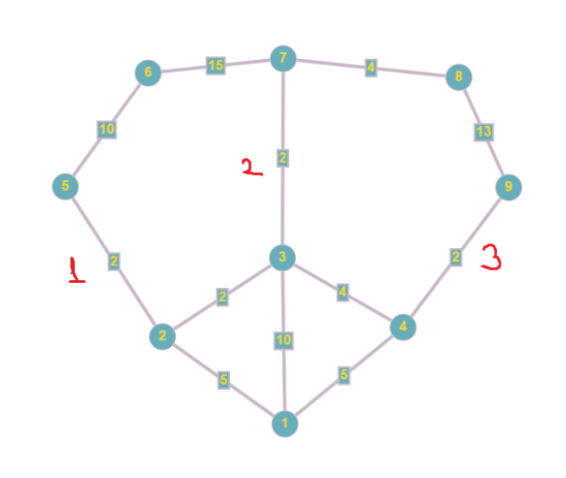
\includegraphics[width=0.7\textwidth]{pic/71.png} }
\end{minipage}


Стартовое время 03:30. Своды мостов:
\begin{enumerate}
\item 03:30 - 03:40
\item 04:05 - 04:15
\item 03:45 - 03:55
\end{enumerate}

---------------

Автор -- Максим Акимцов, M3307
